\documentclass[border=10pt]{standalone}

\usepackage{tikz}
\usepackage{tikzsymbols}
\usetikzlibrary{calc,patterns,shapes.geometric}

\def\centerarc[#1](#2)(#3:#4:#5){\draw[#1] ($(#2)+({#5*cos(#3)},{#5*sin(#3)})$) arc (#3:#4:#5);}

\begin{document}
	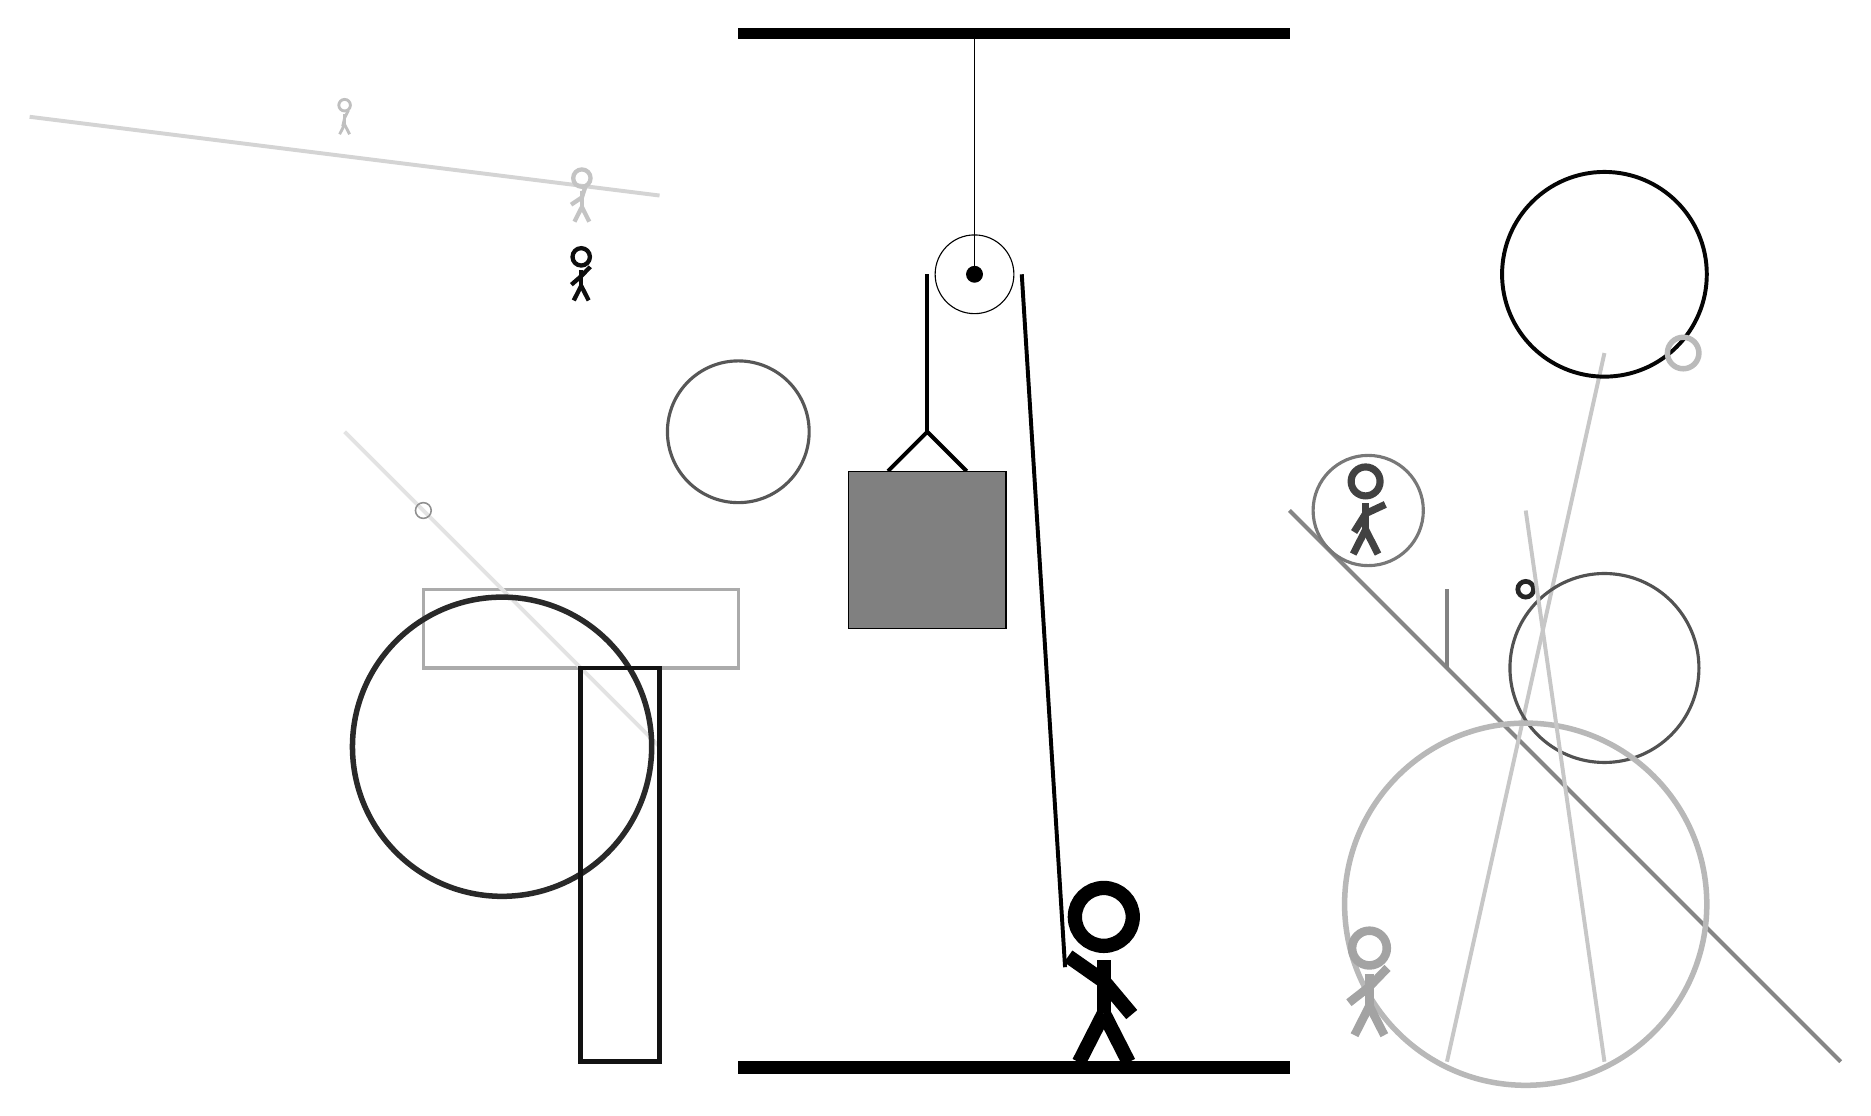
\begin{tikzpicture}
		%%%%% START %%%%%
		
		\draw[fill=black] (-2, 10) rectangle (5, 10.125);
		
		\draw (1, 7) circle (0.5);
		\draw[fill=black] (1, 7) circle (0.1);
		\draw (1, 10) -- (1, 7);
		
		\draw[line width=0.5mm] (-0.1, 4.5) -- (0.4, 5.0) -- (0.9, 4.5);
		\draw[fill=black!50] (-0.6, 4.5) rectangle (1.4, 2.5);
		
		\draw[line width=0.4mm, color=black!33] (-2, 2) rectangle (-6, 3);
		
		\draw[line width=0.5mm, color=black!11](-3, 1) -- (-7, 5);
		\draw[line width=0.5mm, color=black!48](5, 4) -- (12, -3);
		\draw [line width=0.7mm, color=black!84](-5, 1) circle (1.9);
		
		\draw [line width=0.2mm, color=black!44](-6, 4) circle (0.1);
		\draw[line width=0.5mm, color=black!17](-3, 8) -- (-11, 9);
		
		\draw [line width=0.4mm, color=black!53](6, 4) circle (0.7);
		\draw[line width=0.5mm, color=black!22](9, 6) -- (7, -3);
		\node[line width=0.7mm, color=black!74] at (6, 4) {\Strichmaxerl[5][58][25]};
		\draw [line width=0.4mm, color=black!68](9, 2) circle (1.2);
		\draw[line width=0.5mm, color=black!49] (7, 3) rectangle (7, 2);
		\draw [line width=0.5mm, color=black!98](9, 7) circle (1.3);
		\node[line width=0.7mm, color=black!23] at (-4, 8) {\Strichmaxerl[3][34][72]};
		\draw [line width=0.4mm, color=black!66](-2, 5) circle (0.9);
		\draw [line width=0.6mm, color=black!85](8, 3) circle (0.1);
		\draw [line width=0.7mm, color=black!27](10, 6) circle (0.2);
		
		\node[line width=0.5mm, color=black!25] at (-7, 9) {\Strichmaxerl[2][77][64]};
		
		\draw [line width=0.7mm, color=black!28](8, -1) circle (2.3);
		\node[line width=0.5mm, color=black!95] at (-4, 7) {\Strichmaxerl[3][41][46]};
		\draw[line width=0.5mm, color=black!22](8, 4) -- (9, -3);
		\draw[line width=0.6mm, color=black!93] (-3, 2) rectangle (-4, -3);
		\node[line width=0.7mm, color=black!36] at (6, -2) {\Strichmaxerl[6][38][46]};
		
		
		\draw[line width=0.5mm] (0.4, 7) -- (0.4, 5.0);
		\centerarc[line width=0.5mm](1, 7)(0:180:0.6);
		\draw[line width=0.5mm](1.6, 7) -- (2.15, -1.8);
		
		\node at (2.6, -1.9) {\Strichmaxerl[10][-35][-50]};
		
		\draw[fill=black] (-2, -3) rectangle (5, -3.15);
		
		%%%%% END %%%%%
	\end{tikzpicture}
\end{document}